\begin{figure}[!h]
    \centering
    \caption{Percolation realisations on a $10 \times 10$ section of $\Z^2$ for 3 different values of $p$}
    \label{fig:3_realisations}
    \minipage{0.32\textwidth}
    \centering
    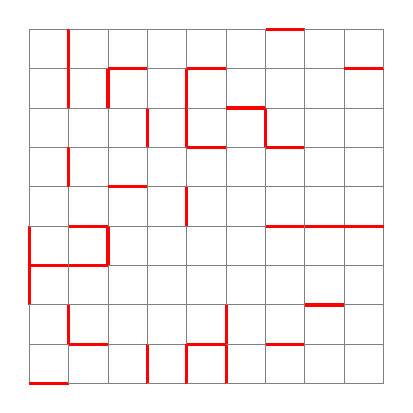
\begin{tikzpicture}
        \def\p{0.2}
        \foreach \x in {0,0.50,...,4.00} {
            \foreach \y in {0,0.50,...,4.00} {
                \pgfmathparse{rnd}
                \ifdim\pgfmathresult pt < \p pt\relax 
                    \draw[red, very thick] (\x, \y) -- (\x, \y + 0.50);
                \else
                    \draw[gray] (\x, \y) -- (\x, \y + 0.50);
                \fi 
                \pgfmathparse{rnd}
                \ifdim\pgfmathresult pt < \p pt\relax
                    \draw[red, very thick] (\x, \y) -- (\x + 0.50, \y);
                \else
                    \draw[gray] (\x, \y) -- (\x + 0.50, \y);
                \fi 
            }
            \pgfmathparse{rnd}
            \ifdim\pgfmathresult pt < \p pt\relax
                \draw[red, very thick] (\x, 4.50) -- (\x + 0.50, 4.50);
            \else
                \draw[gray] (\x, 4.50) -- (\x + 0.50, 4.50);
            \fi
            \pgfmathparse{rnd}
            \ifdim\pgfmathresult pt < \p pt\relax
                \draw[red, very thick] (4.50, \x) -- (4.50, \x + 0.50);
            \else
                \draw[gray] (4.50, \x) -- (4.50, \x + 0.50);
            \fi
        }
    \end{tikzpicture}
    \caption*{$p = 0.2$}
    \endminipage\hfill
    \minipage{0.32\textwidth}
    \centering
    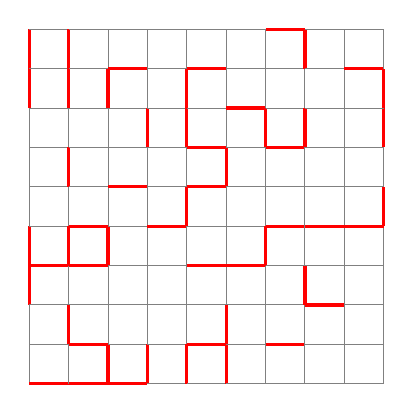
\begin{tikzpicture}
        \def\p{0.3}
        \foreach \x in {0,0.50,...,4.00} {
            \foreach \y in {0,0.50,...,4.00} {
                \pgfmathparse{rnd}
                \ifdim\pgfmathresult pt < \p pt\relax 
                    \draw[red, very thick] (\x, \y) -- (\x, \y + 0.50);
                \else
                    \draw[gray] (\x, \y) -- (\x, \y + 0.50);
                \fi 
                \pgfmathparse{rnd}
                \ifdim\pgfmathresult pt < \p pt\relax
                    \draw[red, very thick] (\x, \y) -- (\x + 0.50, \y);
                \else
                    \draw[gray] (\x, \y) -- (\x + 0.50, \y);
                \fi 
            }
            \pgfmathparse{rnd}
            \ifdim\pgfmathresult pt < \p pt\relax
                \draw[red, very thick] (\x, 4.50) -- (\x + 0.50, 4.50);
            \else
                \draw[gray] (\x, 4.50) -- (\x + 0.50, 4.50);
            \fi
            \pgfmathparse{rnd}
            \ifdim\pgfmathresult pt < \p pt\relax
                \draw[red, very thick] (4.50, \x) -- (4.50, \x + 0.50);
            \else
                \draw[gray] (4.50, \x) -- (4.50, \x + 0.50);
            \fi
        }
    \end{tikzpicture}
    \caption*{$p = 0.3$}
    \endminipage\hfill
    \minipage{0.32\textwidth}
    \centering
    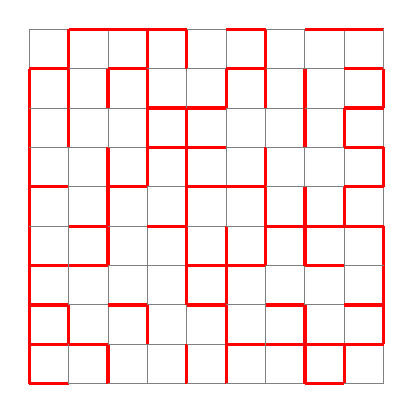
\begin{tikzpicture}
        \def\p{0.6}
        \foreach \x in {0,0.50,...,4.00} {
            \foreach \y in {0,0.50,...,4.00} {
                \pgfmathparse{rnd}
                \ifdim\pgfmathresult pt < \p pt\relax 
                    \draw[red, very thick] (\x, \y) -- (\x, \y + 0.50);
                \else
                    \draw[gray] (\x, \y) -- (\x, \y + 0.50);
                \fi 
                \pgfmathparse{rnd}
                \ifdim\pgfmathresult pt < \p pt\relax
                    \draw[red, very thick] (\x, \y) -- (\x + 0.50, \y);
                \else
                    \draw[gray] (\x, \y) -- (\x + 0.50, \y);
                \fi 
            }
            \pgfmathparse{rnd}
            \ifdim\pgfmathresult pt < \p pt\relax
                \draw[red, very thick] (\x, 4.50) -- (\x + 0.50, 4.50);
            \else
                \draw[gray] (\x, 4.50) -- (\x + 0.50, 4.50);
            \fi
            \pgfmathparse{rnd}
            \ifdim\pgfmathresult pt < \p pt\relax
                \draw[red, very thick] (4.50, \x) -- (4.50, \x + 0.50);
            \else
                \draw[gray] (4.50, \x) -- (4.50, \x + 0.50);
            \fi
        }
    \end{tikzpicture}
    \caption*{$p = 0.6$}
    \endminipage\hfill
\end{figure}